\documentclass[a4paper,12pt]{article}

\usepackage[utf8]{inputenc}
\usepackage{geometry}

\geometry{
    left=1cm,
    right=1cm,
    top=1.5cm,
    bottom=2.5cm
}

\usepackage{setspace}
\usepackage{tikz}
\usetikzlibrary{trees}
\usetikzlibrary{arrows}
\usetikzlibrary{arrows.meta}

\begin{document}

\begin{center}
    
    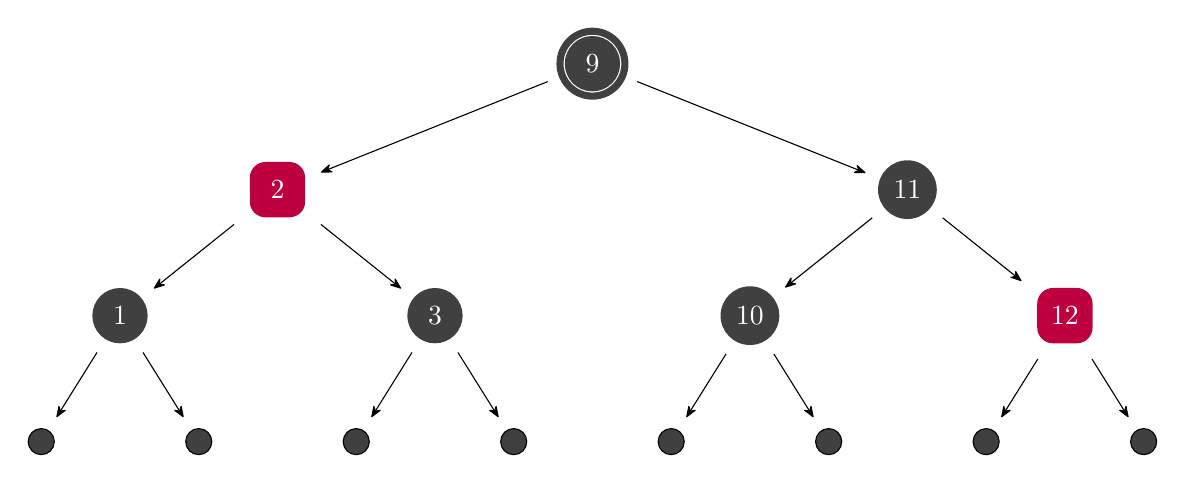
\begin{tikzpicture}[level distance=1.6cm,
        level 1/.style={sibling distance=8cm},
        level 2/.style={sibling distance=4cm},
        level 3/.style={sibling distance=2cm},
        node distance=3.5cm,
        ->,-{Stealth[round,open,fill=black]},
        blackNode/.style = {shape=circle,fill=darkgray,text=white,minimum size=2em,outer sep=0.2cm},
        redNode/.style = {fill=purple,text=white,rounded corners=2mm,minimum size=2em,outer sep=0.2cm},
        endNode/.style = {shape=circle,draw=black,fill=darkgray,text=white,outer sep=0.2cm},
        innerBlackNode/.style = {shape=circle,fill=darkgray,text=white,minimum size=2em}, % inner node for double-black-state
        innerRedNode/.style = {shape=circle,fill=purple,text=white,minimum size=2em}, % inner node for red-black-state
        outerNode/.style = {shape=circle,very thick,draw=darkgray,fill=white,outer sep=0.2cm, inner sep=-0.6mm, distance=0.01cm,line width=0.9mm}
        ]
        \node[outerNode] {\tikz\node[innerBlackNode]{9};}
        child {node[redNode] {2} 
        child {node[blackNode] {1}
        child{node[endNode] {}}
        child{node[endNode] {}}}
        child {node[blackNode] {3}
        child{node[endNode] {}}
        child{node[endNode] {}}}}
        child {node[blackNode] {11} 
        child {node[blackNode] {10} 
        child {node[endNode] {}} 
        child {node[endNode] {}}} 
        child {node[redNode] {12} 
        child {node[endNode] {}} 
        child {node[endNode] {}}}};
    \end{tikzpicture}

    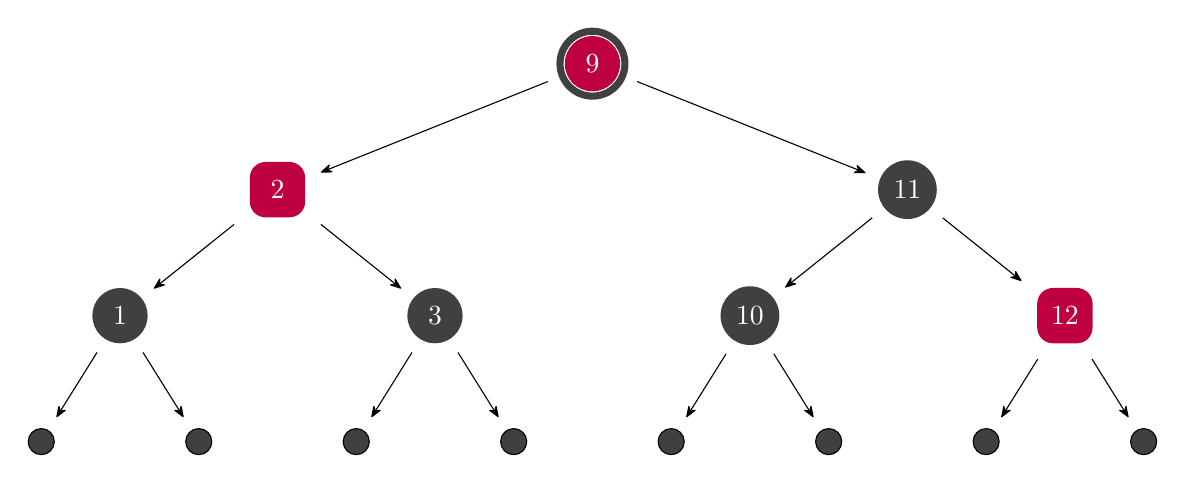
\begin{tikzpicture}[level distance=1.6cm,
        level 1/.style={sibling distance=8cm},
        level 2/.style={sibling distance=4cm},
        level 3/.style={sibling distance=2cm},
        node distance=3.5cm,
        ->,-{Stealth[round,open,fill=black]},
        blackNode/.style = {shape=circle,fill=darkgray,text=white,minimum size=2em,outer sep=0.2cm},
        redNode/.style = {fill=purple,text=white,rounded corners=2mm,minimum size=2em,outer sep=0.2cm},
        endNode/.style = {shape=circle,draw=black,fill=darkgray,text=white,outer sep=0.2cm},
        innerBlackNode/.style = {shape=circle,fill=darkgray,text=white,minimum size=2em}, % inner node for double-black-state
        innerRedNode/.style = {shape=circle,fill=purple,text=white,minimum size=2em}, % inner node for red-black-state
        outerNode/.style = {shape=circle,very thick,draw=darkgray,fill=white,outer sep=0.2cm, inner sep=-0.6mm, distance=0.01cm,line width=0.9mm}
        ]
        \node[outerNode] {\tikz\node[innerRedNode]{9};}
        child {node[redNode] {2} 
        child {node[blackNode] {1}
        child{node[endNode] {}}
        child{node[endNode] {}}}
        child {node[blackNode] {3}
        child{node[endNode] {}}
        child{node[endNode] {}}}}
        child {node[blackNode] {11} 
        child {node[blackNode] {10} 
        child {node[endNode] {}} 
        child {node[endNode] {}}} 
        child {node[redNode] {12} 
        child {node[endNode] {}} 
        child {node[endNode] {}}}};
    \end{tikzpicture}

    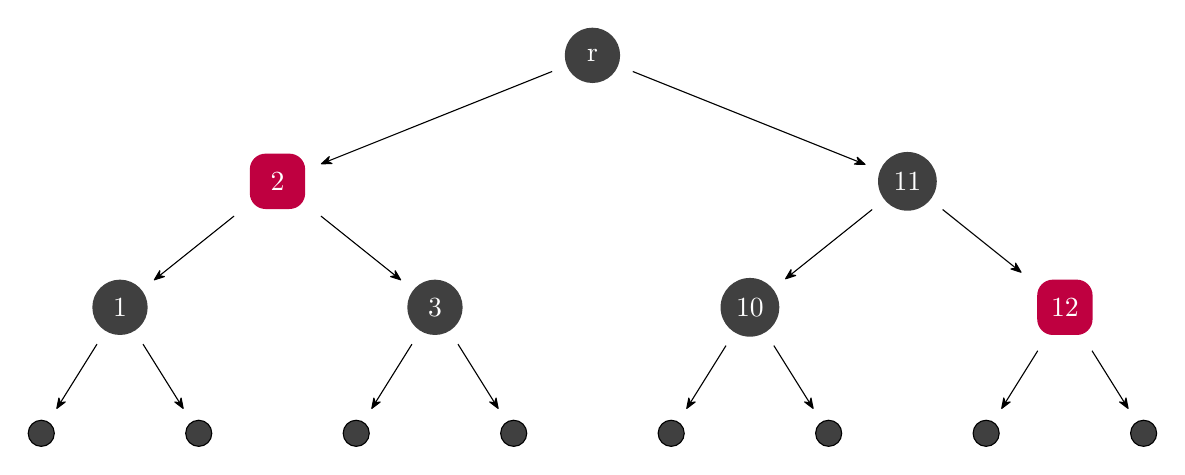
\begin{tikzpicture}[level distance=1.6cm,
        level 1/.style={sibling distance=8cm},
        level 2/.style={sibling distance=4cm},
        level 3/.style={sibling distance=2cm},
        node distance=3.5cm,
        ->,-{Stealth[round,open,fill=black]},
        blackNode/.style = {shape=circle,fill=darkgray,text=white,minimum size=2em,outer sep=0.2cm},
        redNode/.style = {fill=purple,text=white,rounded corners=2mm,minimum size=2em,outer sep=0.2cm},
        endNode/.style = {shape=circle,draw=black,fill=darkgray,text=white,outer sep=0.2cm},
        innerBlackNode/.style = {shape=circle,fill=darkgray,text=white,minimum size=2em}, % inner node for double-black-state
        innerRedNode/.style = {shape=circle,fill=purple,text=white,minimum size=2em}, % inner node for red-black-state
        outerNode/.style = {shape=circle,very thick,draw=darkgray,fill=white,outer sep=0.2cm, inner sep=-0.6mm, distance=0.01cm,line width=0.9mm}
        ]
        \node[blackNode] {r}
        child {node[redNode] {2} 
        child {node[blackNode] {1}
        child{node[endNode] {}}
        child{node[endNode] {}}}
        child {node[blackNode] {3}
        child{node[endNode] {}}
        child{node[endNode] {}}}}
        child {node[blackNode] {11} 
        child {node[blackNode] {10} 
        child {node[endNode] {}} 
        child {node[endNode] {}}} 
        child {node[redNode] {12} 
        child {node[endNode] {}} 
        child {node[endNode] {}}}};
    \end{tikzpicture}
\end{center}
    
\end{document}